\documentclass[12pt]{article}
\usepackage[margin=2.5cm]{geometry}
\usepackage{titling}
\usepackage{enumerate}
\usepackage{graphicx}
\usepackage{mdframed}
\predate{}
\postdate{}

\begin{document}
\title{Lab 2: Introduction to Object-Oriented Programming}
\date{}
\maketitle

\section*{1) Review: Working with tweets}
Your first task is to download the Twitter starter code (tweet.py) the document
into your \textbf{lab2} folder, and open it in PyCharm.

\bigskip

\noindent Review the code from class, and if you have any questions, ask your TA.

\bigskip

\noindent Then, complete each of the TODOs found in that file in the following
order (we’ve arranged these roughly by difficulty).

\bigskip

\begin{enumerate}[1.]
    \item Implement the \textbf{User.verbosity} method.
    \item Discuss with your partner which class the \textbf{retweet} function
    should go into,
    and then move it. (You’ll have to make some minor modifications to the code
    as well.)
    \item Implement the \textbf{User.hack} method.
\end{enumerate}

\bigskip

\section*{2) Designing Classes}

Create a new Python file in your lab2 folder and name it \textbf{registry.py}.
Your task is to perform an object-oriented analysis of a problem specification,
outlined in the steps below.

\bigskip

\textbf{Note:} design is often harder and more time-consuming than implementation!
Work with a partner, and don’t be afraid to take up the rest of the lab time to
get a really solid design done. You’ll find that if you spend your efforts today
on the class design, actually implementing your design will be comparatively
straight-forward.

\bigskip

\textbf{Don’t begin implementation until your design is complete.}

\begin{enumerate}[1.]
\item \textit{Read the problem description.}

Download \textbf{specs.txt} (See Figure ~\ref{fig:specsText}) the document into your \textbf{lab2} folder and read
through the problem description.

\begin{figure}
    \begin{mdframed}
        Race Registry

        =============

        \bigskip

        Context: a system for organizing a 5K running race.

        \bigskip

        When runners register for a race, they provide their name, email address and
        their speed category. A speed category indicates how quickly they estimate that
        they can finish the race. This allows organizers to start the runners in groups
        of roughly equivalent running speed so that faster runners aren't stuck behind
        slower runners. The possible speed categories are: under 20 minutes, under 30
        minutes, under 40 minutes, and 40 minutes or over. We need to be able get a list
        of runners in a given speed category. We also need to be able to look up a
        runner to find their speed category. Finally, a runner should be able to change
        their email address and speed category, or withdraw from the race entirely.

    \end{mdframed}
    \caption{specs.txt}
    \label{fig:specsText}
\end{figure}

\item \textit{Decide what classes you need to design.}

In a basic object-oriented design, each class usually models some noun in the
problem description—but not every noun needs a class to model it. For example,
an email address can be modelled by a simple str.

\bigskip

The one class you need for sure is a class to represent the race registry as a
whole. You can design a reasonable solution that has only that class. Decide
 whether you wish to have any other classes.

\item \textit{Sample usage.}

Next, picture how your class(es) will be used by writing some doctests in the class
docstring of one of your new classes. Your doctests should illustrate the following
behaviour:

\begin{itemize}
    \item Create a race registry.
    \item Register the following runners:
    \begin{itemize}
        \item Gerhard (with time under 40 minutes)
        \item Tom (with time under 30 minutes)
        \item Toni (with time under 20 minutes)
        \item Margot (with time under 30 minutes)
        \item Gerhard again (with time under 30 minutes—he’s gotten faster)
        \item Report the runners in the speed category of under 30 minutes.
    \end{itemize}
\end{itemize}

\bigskip

\textbf{Remember, you haven’t written the class(es) yet!}

Just like function doctests help illustrate the purpose of a function, your class
docstring helps the user (and yourself!) understand how your class should be used.

\item \textit{Designing the interface.}

Use \textbf{Part 1} of the Class Design Recipe the document to create the public
interface of each class.

(You’ve already started doing this in the previous step.) Note that this involves
a lot of documentation and writing of basic examples and tests, but still no
implementation whatsoever. That will come later.

\bigskip

This analysis will require a fair amount of thought. Don’t worry about getting it
completely right. If you find any ambiguities in the specifications, write them
down, and try to come up with a solution you think is reasonable.

\bigskip

A good skill to develop in this course is identifying ambiguities and proposing
multiple solutions for such ambiguities in problem descriptions you receive.
There’s no “one right answer” to this task!

\end{enumerate}

\bigskip

\section*{3) Implementing Your Design}

If you still have time, take your design and implement all of the methods in each
of the classes you defined.

\bigskip

\noindent We’ve provided code in the “main” block at the bottom of the file to
run \textbf{doctest} to check your doctest examples. You should have already
written a doctest example in your class docstring by following the above instructions;
make sure you add some further examples to individual methods to help check the
correctness of your code.

\bigskip

\section*{4) Extra exercises for later}

\subsection*{More small exercises}
Here are some additional exercises (See figure ~\ref{fig:additionalExercise}) the
document in designing and implementing classes. Each section in that file is a
problem description for you to model using an object-oriented design.

\bigskip


\begin{figure}
    \begin{mdframed}
        Fraction

        ========

        \bigskip

        Context: a calculator app

        \bigskip

        We need to be able to multiply fractions, and the print them in their decimal
        form. Fractions, of course have a numerator and a denominator. They need not be
        in their simplest form, for example, we could have 8/2, or 6/8.

        \bigskip

        Player

        ======

        \bigskip

        Context: an app for a game like 2048 or PacMan, where players get a score each
        time they play.

        \bigskip

        A player has a name and a history of the last 100 scores they've achieved in the
        game. We need to keep track of new scores they get so we can determine their top
        score and their average score on their most recent n games, where n is some
        positive whole number.

        \bigskip

        Candyland Board

        ===============

        \bigskip

        Context: The Candyland board game

        \bigskip

        Candyland is a very simple children's game for two players. The board has spaces
        from 0 to 100. On their turn, a player advances a certain number of spaces. The
        first player to reach spot 100 wins. We need to keep track of where the players
        are so that we can report on the location of the two players whenever needed.
        We also want to be able to find out who the winner is: either one of the
        players, both if it's a tie, or no one if the game isn't over yet.

        \bigskip

        Flight Roster

        =============

        \bigskip

        Context: An airline reservation system

        \bigskip

        Each seat has a unique name, like "17C" and is either in business class or
        economy. Passengers have booking IDs (a mix of letters and numbers). When they
        book a seat, they request their preferred class (business or economy) and are
        given any seat in that class. If the class is full, their booking is
        unsuccessful. This airline gives passengers no choice about their specific seat.
        We want to be able to report on how full a flight is: the percentage of seats
        that are booked in economy, in business class, and overall.

    \end{mdframed}
    \caption{additional\_exercise.txt}
    \label{fig:additionalExercise}
\end{figure}

\bigskip

\subsection*{Object-oriented analysis}
As the problems get larger, it becomes more important to be able to focus on high
level design before getting into details. We can record a high-level design with
a simple drawing. Here is a design for our Twitter example the document
in this style (see Figure ~\ref{fig:uml}).

\bigskip

\begin{figure}
    \begin{center}
    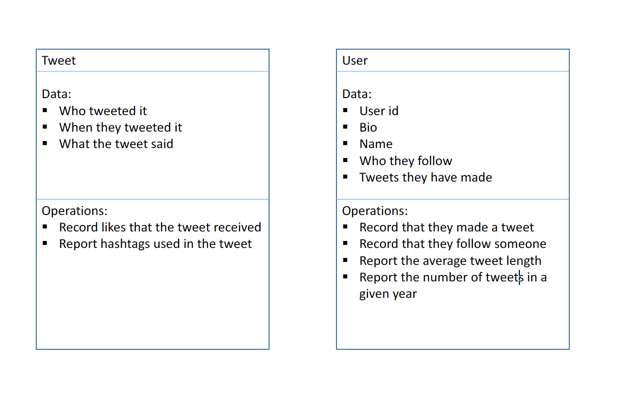
\includegraphics[width=0.8\linewidth]{../images/lab_2/uml.png}
    \end{center}
    \caption{Design for twitter example}
    \label{fig:uml}
\end{figure}

\bigskip

\noindent Notice that this drawing omits details such as what type we should use for each
piece of data, what parameters each method should have, and so on. We can decide
on these later, once we have settled on the overall design.

\begin{itemize}
    \item Read the specifications for this larger problem in \textit{specs\_larger.txt}
    (see figure ~\ref{fig:specsLargerText})the document. Circle the nouns and underline
    the verbs.

    \bigskip

    \begin{figure}
        \begin{mdframed}
            Doctor's Office

            ===============

            \bigskip

            A doctor's office needs software for scheduling appointments. It is a large
            practise with 10 to 15 doctors and several thousand patients. Patients
            can make an appointment with a doctor, and all appointments last 1 hour.
            Doctors schedule blocks of time when they are available for appointments.
            Each patient has a primary doctor. If their primary doctor is available on t
            he hour and day when they wish to book they must see them; otherwise, they
            can see any doctor. A patient may cancel an appointment,but if they cancel
            more than 10, they are no longer allowed to book appointments (ever!).
            Doctors can cancel a block of time when they had said they were available;
            any patients who had appointments during that block get rescheduled at the
            earliest possible time, regardless of which doctor they get.
        \end{mdframed}
        \caption{specs\_larger.txt}
        \label{fig:specsLargerText}
    \end{figure}
\end{itemize}

\bigskip

Using the same diagram style as in the example above, come up with a design for
this software. There is a lot of judgment involved, and there are multiple good
solutions. The point here is to think about and debate some options, and start to
get comfortable with the process.

\end{document}
